%%%%%%%%%%%%%%%%%%%%%%%%%%%%%%%%%%%%%%%%%%%%%%%%%%%%%%%%%%%%%%%%%%%%%%%%%%%%%%%%%%%%%%%%%%%%%%%%%%%%%%%%%%%%%%%%%%%%%%%%%%%%%%%%%%%%%%%%%%%%%%%%%%%%%%%%%%%
% This is just an example/guide for you to refer to when submitting manuscripts to Frontiers, it is not mandatory to use Frontiers .cls files nor frontiers.tex  %
% This will only generate the Manuscript, the final article will be typeset by Frontiers after acceptance.   
%                                              %
%                                                                                                                                                         %
% When submitting your files, remember to upload this *tex file, the pdf generated with it, the *bib file (if bibliography is not within the *tex) and all the figures.
%%%%%%%%%%%%%%%%%%%%%%%%%%%%%%%%%%%%%%%%%%%%%%%%%%%%%%%%%%%%%%%%%%%%%%%%%%%%%%%%%%%%%%%%%%%%%%%%%%%%%%%%%%%%%%%%%%%%%%%%%%%%%%%%%%%%%%%%%%%%%%%%%%%%%%%%%%%

%%% Version 3.4 Generated 2018/06/15 %%%
%%% You will need to have the following packages installed: datetime, fmtcount, etoolbox, fcprefix, which are normally inlcuded in WinEdt. %%%
%%% In http://www.ctan.org/ you can find the packages and how to install them, if necessary. %%%
%%%  NB logo1.jpg is required in the path in order to correctly compile front page header %%%

\documentclass[utf8, a4paper, final, crop]{frontiersSCNS} % for Science, Engineering and Humanities and Social Sciences articles
%\documentclass[utf8]{frontiersHLTH} % for Health articles
%\documentclass[utf8]{frontiersFPHY} % for Physics and Applied Mathematics and Statistics articles


%\usepackage[utf8]{inputenc}
%\usepackage[english]{babel}
%\usepackage{minted}  % for styling python code

% Default fixed font does not support bold face
\DeclareFixedFont{\ttb}{T1}{txtt}{bx}{n}{11} % for bold
\DeclareFixedFont{\ttm}{T1}{txtt}{m}{n}{11}  % for normal

% Custom colors
\usepackage{color}
\definecolor{deepblue}{rgb}{0,0,0.5}
\definecolor{deepred}{rgb}{0.6,0,0}
\definecolor{deepgreen}{rgb}{0,0.5,0}

\usepackage{listings}  % for styling python code

% Python style for highlighting
\newcommand\pythonstyle{\lstset{
language=Python,
basicstyle=\ttm,
otherkeywords={self},             % Add keywords here
keywordstyle=\ttb\color{deepblue},
emph={MyClass,__init__, False,True},          % Custom highlighting
emphstyle=\ttb\color{violet},    % Custom highlighting style
stringstyle=\ttfamily\color{deepgreen},
frame=tlrb,%tb,                         % Any extra options here
showstringspaces=false            % 
}
\lstset{literate=%
   *{0}{{{\color{deepred}0}}}1
    {1}{{{\color{deepred}1}}}1
    {2}{{{\color{deepred}2}}}1 %\color{red!20!violet}
    {3}{{{\color{deepred}3}}}1
    {4}{{{\color{deepred}4}}}1
    {5}{{{\color{deepred}5}}}1
    {6}{{{\color{deepred}6}}}1
    {7}{{{\color{deepred}7}}}1
    {8}{{{\color{deepred}8}}}1
    {9}{{{\color{deepred}9}}}1
}
}

% Python environment
\lstnewenvironment{python}[1][]
{
\pythonstyle
\lstset{#1}
}
{}
\newcommand{\pythoninline}[1]{\pythonstyle\lstinline[columns=fixed]{#1}}

%\lstMakeShortInline[columns=fixed]|

%\setcitestyle{square} % for Physics and Applied Mathematics and Statistics articles
\usepackage{url,hyperref,lineno,microtype,subcaption}
\usepackage[onehalfspacing]{setspace}

%\linenumbers


% Leave a blank line between paragraphs instead of using \\


\def\keyFont{\fontsize{8}{11}\helveticabold }
\def\firstAuthorLast{Bougacha {et~al.}} %use et al only if is more than 1 author

\def\Authors{Salma Bougacha\,$^{1,2,*}$, Nachiket Nadkarni\,$^{1}$, Marina Celestine\,$^{1}$, Cl\'ement Garin\,$^{1}$, and Marc Dhenain\,$^{1}$}
% Affiliations should be keyed to the author's name with superscript numbers and be listed as follows: Laboratory, Institute, Department, Organization, City, State abbreviation (USA, Canada, Australia), and Country (without detailed address information such as city zip codes or street names).
% If one of the authors has a change of address, list the new address below the correspondence details using a superscript symbol and use the same symbol to indicate the author in the author list.
\def\Address{$^{1}$Neurodegenerative Dis. Lab., MIRCen, CEA, Fontenay aux Roses Cedex, France \\
$^{2}$U1077, Cyceron, INSERM, Caen, France
%$^{2}$Laboratory X, Institute X, Department X, Organization X, City X , State XX (only USA, Canada and Australia), Country X  
}
% The Corresponding Author should be marked with an asterisk
% Provide the exact contact address (this time including street name and city zip code) and email of the corresponding author
\def\corrAuthor{Corresponding Author}

\def\corrEmail{salma.bougacha@hotmail.com}




\begin{document}
%\onecolumn
\firstpage{1}

\title[Sammba-MRI]{Sammba-MRI: a library for processing SmAll MaMmals BrAin MRI data in Python} 
%{Sammba-MRI: a library for processing SmAll MaMmals neuroimaging data in Python} 


\author[\firstAuthorLast ]{\Authors} %This field will be automatically populated
\address{} %This field will be automatically populated
\correspondance{} %This field will be automatically populated

\extraAuth{}% If there are more than 1 corresponding author, comment this line and uncomment the next one.
%\extraAuth{corresponding Author2 \\ Laboratory X2, Institute X2, Department X2, Organization X2, Street X2, City X2 , State XX2 (only USA, Canada and Australia), Zip Code2, X2 Country X2, email2@uni2.edu}


\maketitle


\begin{abstract}
Small mammals neuroimaging offers incredible opportunities to investigate structural and
functional aspects of the brain. Many tools have been developed in the last decade to analyze
small animal data, but current softwares are less mature than the available tools that process
human brain data. The Python package sammba-MRI (SmAll MaMmals BrAin MRI in Python;
http://sammba-mri.github.io) is designed to allow flexible and efficient use of existing methods and
enables fluent scriptable analysis workflows, from DICOM conversion to results visualization.
%%% Leave the Abstract empty if your article does not require one, please see the Summary Table for full details.
%For full guidelines regarding your manuscript please refer to \href{http://www.frontiersin.org/about/AuthorGuidelines}{Author Guidelines}.
%As a primary goal, the abstract should render the general significance and conceptual advance of the work clearly accessible to a broad readership. References should not be cited in the abstract. Leave the Abstract empty if your article does not require one, please see \href{http://www.frontiersin.org/about/AuthorGuidelines#SummaryTable}{Summary Table} for details according to article type. 


\tiny
 \keyFont{ \section{Keywords:} Processing pipeline, MRI, registration, small animal Neuroimaging, Python } %All article types: you may provide up to 8 keywords; at least 5 are mandatory.
\end{abstract}

\section{Introduction}

Small mammals neuroimaging allows to investigate structural and functional aspects in animal models of the healthy and diseased brain. Challenges in small animal MRI include [...].
Technical advances entail increasing data resolution, sample size, and meta-information complexity. 
The changing data properties call for more advanced statistical methods that scale naturally to the high-dimensional regime, are inter-operable in complex processing pipelines, and can better exploit modern multiprocessing architectures than predominant methods.
%
%For Original Research Articles , Clinical Trial Articles, and Technology Reports , the introduction should be succinct, with no subheadings. For Case Reports the Introduction should include symptoms at presentation, physical exams and lab results.
%

\section{Tools: nipy ecosystem and neuroimaging software packages}

With its mature scientific stack, Python is a growing contender
in the landscape of neuroimaging data analysis with tools such as
Nipy (Millman and Brett, 2007) or Nipype (Gorgolewski et al.,
2011). The scientific Python libraries used in this paper are:
%
%For requirements for a specific article type please refer to the Article Types on any Frontiers journal page. Please also refer to  \href{http://home.frontiersin.org/about/author-guidelines#Sections}{Author Guidelines} for further information on how to organize your manuscript in the required sections or their equivalents for your field
% For Original Research articles, please note that the Material and Methods section can be placed in any of the following ways: before Results, before Discussion or after Discussion.
%

\section{Code design}

All pipelines rely on scikit-learn transformers.
Graphical or interactive interfaces are avoided, as
they impede reproducibility, encumber the depen-
dency graph, and reduce the sustainability of the
project.

\section{Preprocessing bricks}

\subsection{DICOM to NIFTI conversion}

Sammba-MRI allows to convert Bruker DICOM files to the standard Nifti-1 
imaging format and extracts extensive information using DCMTK. 
Bruker files conversion is an active development field,
with various available tools handling DICOM \citeauthor{dicomifier} or
not \citeauthor{bru2nii, bruker2nifti}.
Finally, ParaVision 360 with the latest patch 1.1 can export the NIFTI format since [...].
%Finally, ParaVision can export the NIFTI format. But, one needs to upgrade to ParaVision 360 with the latest patch 1.1. Most users using PV 6 are still left behind. So, Bru2Nii is still needed before Bruker upgrading PV 6 to support NIFTI.
Our implementation is meant to be a light helper function, allowing to 
handle the conversion on the fly. It has been tested only for Paravision 6
and a limited number of imaging sequences.

\subsection{Bias field correction}

Intensity non-uniformity modelling is essential in preclinical studies
because the intensity gradient corrupting MR images becomes
particularly [important, pronounced] at high field strengths \citep{boyes2008intensity}.
Sammba-MRI relies on AFNI 3dUnifize to correct for intensity bias in
anatomical images, and on N4BiasFieldCorrection function
of the ANTs package \citep{tustison2010n4itk}
for the other modalities. 3dUnifize is also used to aid brain extraction,
as detailed in the following paragraph.

% from Power Phd
%A smoothly-varying, hardware-induced, low-frequency intensity gradient often corrupts MR images (Sled & Pike, 1998). This is caused by inhomogeneity of the scanner’s B0 field, variable sensitivity of the receiver coils, or inhomogeneity of the radiofrequency pulse, which can be induced via non-uniformity of the transmission coil or via electromagnetic interactions and distortions by the subjects themselves (Lewis & Fox, 2004). As this effect becomes especially pronounced at high field strengths (Boyes et al.,2008), intensity non-uniformity modelling is essential in preclinical studies. NUC improves automated tissue classifications and image registration (Sled & Pike, 1998; Van Leemput et al., 1999; Lewis & Fox, 2004). Locally adaptive NUC algorithms, such as N3, have been shown to outperform nonadaptive methods (Arnold et al., 2001). I initially employed N3 (Sled et al., 1998), and later the N4ITK (N4) algorithm (Tustison et al., 2010), found to reliably correct bias at high field strengths, using 200 iterations; 256 histogram bins; a 0.15mm FWHM Gaussian kernel to model the bias field; subsampling factor 4 (for high-resolution, ex vivo images) or 2 (for lower-resolution in vivo images). NUC is further refined during the iterative expectation maximisation steps of tissue segmentation. In neither technique is the image resampled; thus image quality is maintained.

\subsection{Brain extraction}

Brain extraction is the critical early step in processing
MRI images from small animals. Various rodent-specific 
automatic software or human adapted tools exist [citations].
We choose to rely on
the LOGISMOS-based graph segmentation \citep{yin2010logimos} based on grayscale mathematical morphology 
%Oguz et al. (2014) followed mathematical morphology operations with an intensity gradient-based graph cut method to constrain the outer surface of a rodent brain mask. This required varying smoothness constraints across the resulting brain surface, and a manually-specified upper bound on the brain volume. 
RATS software  \citep{oguz2014rats} because
of its good performance across a wide range of datasets and its high 
speed.
%and the template-based skullstripper \citep{delora2016simple}.
An alternative to the free but non-open source RATS tool is also 
available, based on an adaptation of the 
human histogram-based brain extraction method of nilearn. 
This method can be used in any pipeline by setting the parameter
 \pythoninline{use_rats_tool} to \pythoninline{False}.
Because severe intensity inhomogeneity can compromise
the skull stripping quality, prior bias field correction with
3dUnifize
is possible [manageable] [can be controlled/ performed within].
The helper function \pythoninline{brain_segmentation_report} allows to
efficiently tune the initial intensity threshold used in bias correction by
producing for a given set of thresholds 5 informative measures
characterizing the extracted mask to bypass for [a wide range] of thresholds time 
consuming visual checks.
The returned features %reflect the masking] quality and 
consist of the total volume of
the extracted mask, its 
anteroposterior length, its right-left width, and its inferior-superior hight as well
as the sample Pearson's product-moment correlation
coefficient between the brain mask image and its reflection
with respect to the estimated mid-sagittal plane
%its symmetry in the mid-sagittal plane 
%inspired from 
\citep{powell2016fully}.

\section{Ready-to-use pipelines}

\subsection{Template matching}

Template matching is a necessary step for group studies.
%
% from Ionas et al
%In order to make any generalizable statements regard- ing brain function and organization, an equivalence between brain areas across individuals needs to be established. This is done by spatial transformation of brain maps in a study to a population or standard reference template.
%
%Several MRI templates exist for mouse
Sammba-MRI registration relies on AFNI's 3dAllineate and 3dQwarp functions to 
estimate linear and non linear transforms respectively between an individual image
and a reference image. Internal parameters of these functions have been optimized for
small animal brains.
We experienced a better performance when linear registration
is performed on brain extracted images and nonlinear warps are computed
using whole head images, and therefore followed this strategy across all the 
registration pipelines.
%on the estimation of a linear transform between the brain extracted images with AFNI's 3dAllineate, followed by the computation of a nonlinear warp between the whole head images with AFNI 3dQwarp.
%with spatial parameters adapted to the mouse brain
\begin{python}
from sammba.registration import 
    TemplateRegistrator

registrator = TemplateRegistrator(
    'dorr_t2.nii.gz',
    brain_volume=400)
registrator.fit('mouse01_t1.nii.gz')
\end{python}

Registration accuracy has been evaluated on Brookhaven's data \citep{ma2008vivo} by 
measuring the correspondence of segmented structures between individual images 
registered 
to their average template and the template itself.
Because the shared individual images have been pre-registered to one reference image, 
they have been submitted to slight random quadratic deformations (Normally 
distributed coefficients with std=$0.1$ mm for translation, $0.1$ degrees for 
rotation, $0.02$ mm for scaling, $0.02$ mm for shear and $0.005$ mm for the remaining $31$ polynomial coefficients) before performing registration.
%
For comparison purposes, registration has been repeated using SPM mouse \citep{sawiak2009spmmouse}.
Regional overlap was measured
between each region in the average atlas and the transformed mice atlases 
using Dice's coefficient.
Figure ~\ref{fig:dices} shows that sammba-MRI registration achieves
high overlap values and outperforms SPM mouse in the majority of cases.

\subsection{Group-wise registration} % Creation of cohort-specific templates
% from Power
%Group-wise registration (GWR) aims to align all images within a common coordinate space, resulting in an average “atlas” image representing the mean group morphology, and deformation fields mapping each voxel to points in the original image space.
%

Studying populations of animals gains precision by the use of cohort-specific 
templates. Sammba-MRI proposes an iterative method to create a fine anatomical 
template from individual structural MRI scans. A first rough template is obtained
by averaging bias corrected head images centred on their respective brain masks barycentres. Then the individual images are registered to this template
and this process of successive registration/averaging is iterated while increasing the number of degrees of 
freedom of the estimated transform and updating the target template. The registrations rely on AFNI linear 
alignment and nonlinear warping, see \citep{nadkarni20193d} for a detailed description of the pipeline. This hopefully allows the creation of high quality
group average templates (Figure ~\ref{fig:mouse_template}). The method adapts to different small animal species, e.g. mouse lemurs %as achieved in 
\citep{nadkarni2018digital}.

%\section{Between-modalities registration}
\subsection{Multi-modal processing}

%TODO: remove where no example
In the context of the increasing use of multimodal imaging, several %modalities
MRI 
%and non MRI 
techniques 
can 
be acquired from small animals, including %and not restricted 
structural imaging with different contrasts, 
%or contrast agents,
%whether by endogenous or exogenous contrast
blood-oxygenation-level-dependent (BOLD) and  arterial spin labeling (ASL) MRI.
%, diffusion-weighted and chemical exchange saturation transfer (CEST) MRI, positron-emission tomography (PET) imaging.
%
%Magnetic resonance (MR) imaging is well known for its noninvasiveness and abundance of image contrasts. Conventional MR imaging contrasts are based on the spin relaxation rates of different body tissues under a static magnetic field and various radiofrequency (RF) pulses. Commonly encountered contrasts include T1, T2, proton density (PD), and T2* [1]. The search for novel image contrasts has been the ever-existing driving force in the MR research community, in order to gain further information on the body’s physiological and pathological conditions. Novel image contrasts have been developed by exploiting different aspects: physical or structural properties (diffusion-weighted imaging [2–4], MR elastography [5, 6], etc.); functional properties (perfusion [7, 8], BOLD [9, 10], resting state fMRI [11, 12], etc.); and chemical composition (MR spectroscopy [13, 14], chemical exchange saturation transfer (CEST) [15–22], etc.).
In addition to the inherent difficulties in intermodality registration \citep{ashburner1997multimodal},
%image artifacts or low resolution can alter
severe image artifacts can corrupt the non anatomical scan
resulting in a low signal-to-noise ratio (SNR).
For instance, the echo 
planar imaging (EPI) %is an ultrafast acquisition 
technique widely used in %diffusion imaging, 
functional MRI and perfusion imaging
suffers nonlinear geometric and intensity distortions caused by static magnetic field 
inhomogeneity that 
worsen at higher field strengths and have a more dramatic impact on small brains
\citep{hong2015evaluation}. 

%Echo planar imaging (EPI) is an ultrafast acquisition technique widely used in diffusion imaging, functional MRI and perfusion imaging. However, it suffers from geometric and intensity distortions caused by static magnetic field inhomogeneity, which is worse at higher field strengths. Such susceptibility artifacts are particularly severe in relation to the small size of the mouse brain. 
%Among the image acquisition pulse sequences, echo planar imaging (EPI) is an ultrafast sequence widely applied to functional MRI (fMRI), diffusion imaging and perfusion imaging. It suffers from geometric and intensity distortions as well as signal dropouts that are caused by static magnetic field inhomogeneity [5], [6], particularly in the through plane direction due to the typically lower resolution than inplane. 
%The issue is especially severe in preclinical imaging. Firstly, the mouse brain is much smaller than the human brain. The same spatial extent of spin displacement affects a much larger portion of the mouse brain. Secondly, field inhomogeneity and hence distortions are proportional to the magnetic field strength. With rodent imaging typically performed at higher magnetic field strengths than human imaging, the artifacts worsen.
%Among the image acquisition pulse sequences, echo planar imaging (EPI) is an ultrafast sequence widely applied to functional MRI (fMRI), diffusion imaging and perfusion imaging. It suffers from geometric and intensity distortions as well as signal dropouts that are caused by static magnetic field inhomogeneity [5], [6], particularly in the phase-encoding direction due to the relatively low pixel bandwidth or in the through plane direction due to the typically lower resolution than inplane. The resultant global and regional distortions are commonly seen near the air-tissue or bone-tissue interfaces, where magnetic susceptibility changes rapidly. The issue is especially severe when translating similar methods to transgenic mouse models to understand disease mechanisms and drug effects. Firstly, the mouse brain is much smaller than the human brain. The same spatial extent of spin displacement affects a much larger portion of the mouse brain. Secondly, field inhomogeneity and hence distortions are proportional to the magnetic field strength. With rodent imaging typically performed at higher magnetic field strengths than human imaging, the artifacts worsen. The geometric distortion will result in localization errors, difficulty in image registration and hence group analysis. The intensity distortion in EPI could also bias the quantitative measures such as relaxivity, diffusivity and perfusion, since quantification of these metrics usually involves nonlinear fitting of the EPI series.
%Among the image acquisition pulse sequences, echo planar imaging (EPI) is an ultrafast sequence widely applied to functional MRI (fMRI), diffusion imaging and perfusion imaging. It suffers from geometric and intensity distortions as well as signal dropouts that are caused by static magnetic field inhomogeneity [5], [6], particularly in the phase-encoding direction due to the relatively low pixel bandwidth or in the through plane direction due to the typically lower resolution than inplane. The resultant global and regional distortions are commonly seen near the air-tissue or bone-tissue interfaces, where magnetic susceptibility changes rapidly. The issue is especially severe when translating similar methods to transgenic mouse models to understand disease mechanisms and drug effects. Firstly, the mouse brain is much smaller than the human brain. The same spatial extent of spin displacement affects a much larger portion of the mouse brain. Secondly, field inhomogeneity and hence distortions are proportional to the magnetic field strength. With rodent imaging typically performed at higher magnetic field strengths than human imaging, the artifacts worsen. The geometric distortion will result in localization errors, difficulty in image registration and hence group analysis. The intensity distortion in EPI could also bias the quantitative measures such as relaxivity, diffusivity and perfusion, since quantification of these metrics usually involves nonlinear fitting of the EPI series.
%One could reduce the signal dropouts seen in gradient echo imaging by incorporating slice shimming, also known as the z-shim technique, into the pulse sequence [7], [8], [9]. However this will prolong the image acquisition time depending on how many z-shim steps used. Spin-echo based acquisition, which is less sensitive to field inhomogeneity, could help to reduce the distortion. However, even with spin-echo EPI (SE-EPI), the geometric and intensity distortions are still significant at high field strengths. The artifact is also echo time (TE) dependent; however, ultrashort TE is difficult to achieve with EPI. Another way is to reduce the echo train length by increasing the bandwidth or using partial Fourier, at the cost of lower SNR and/or spatial resolution. Echo train length can also be reduced by multi-shot EPI, but the acquisition time will be longer and the phase error between shots would introduce additional artifacts. Applying localized susceptibility matching materials near the air/bone-tissue interfaces can reduce the regional magnetic inhomogeneity, though it will be difficult for regions away from the skin [10]. Alternatively, postprocessing methods can be applied to reduce the distortions.
%Several EPI distortion correction algorithms have been proposed and demonstrated successfully in human studies at lower fields. The most common way is based on magnetic field mapping. A field map, measured by the phase differences of two gradient echo images acquired with different TEs, describes the spatial variation of the magnetic field, from which a voxel displacement map can be calculated and used to unwrap the distorted EPI images [11], [12]. The main drawback of this technique is the separate acquisition of the multiecho images. Subject movement between the field mapping and EPI acquisition could render the field map inaccurate. In addition, the phase unwrapping process is sensitive to noise; therefore the field map in regions of low SNR is unreliable. Alternatively, one can acquire a phase-encoded multi-reference scan to estimate the magnitude and phase errors due to the field inhomogeneity, and then use that to correct the EPI artifact [13].
%Geometric distortions can also be corrected for by nonlinear registration to an anatomically correct image, typically acquired by fast spin echo (FSE). The deformation field could be calculated by minimizing the least squared differences of intensity [14] or log-intensity [15] between the distorted EPI and anatomical images. The undistortion performance highly depends on the registration algorithm, implementation, and parameter optimization. Besides, it only corrects for geometric distortion but not the intensity distortion, which may still result in quantification error.

Sammba-MRI offers 4 different pipelines to perform coregistration
between anatomical scans and other modalities, correcting for geometric 
distortions if needed.
\begin{python}
from sammba.registration import 
    Coregistrator
coregistrator = Coregistrator(
    brain volume =400)
\end{python}
All registration pipelines start with bias filed correction for the anatomical scan
and the modality of interest. 
%\subsubsection{Registration with anatomical}

\subsubsection{Rigid-body registration}
Since orientation is correctly handled through the DICOM to NIFTI conversion,
the anatomical image is first reoriented to match the modality of interest.
Both images then undergo intensity unifization and brain extraction.
A rigid body
transform that minimizes normalized mutual information [between]
between the brain extracted images is estimated and applied to the whole head images.
\begin{python}
coregistrator.fit_anat(
    'mouse01_t1.nii.gz')
coregistrator.fit_modality(
    'mouse01_t2.nii.gz')
\end{python}
%\begin{minted}
%[frame=lines, framesep=2mm, baselinestretch=1.2, bgcolor=LightGray, fontsize=\footnotesize, linenos]{python}
%coregistrator.fit_anat('t1.nii.gz')
%coregistrator.fit_modality('t2.nii.gz', modality='t2')
%\end{minted}

\subsubsection{Reorientation-only}

It is possible that the source or/and the reference
images are of insufficient quality to correctly estimate a rigid body transform
(see figure ...). In this case,
assuming that the head motion between the two acquisitions is low, it is [better]
to only reorient the anatomical image to match the modality of interest.
\begin{python}
coregistrator.fit_anat('t1.nii.gz')
coregistrator.fit_modality(
    't2.nii.gz',
    reorient_only=True)
\end{python}

\subsubsection{Resting state BOLD fMRI processing}

BOLD scans are preprocessed using the same usual steps for human data
with optional slice timing correction, bias field correction, realignment to the 
first volume
and computation of the temporal mean of all the volumes.
The corresponding structural scan is then registered to the average BOLD scan.
Since this is a critical step, the user can choose
either to pursue with human-like pipeline by estimating a rigid body functional-to-
structural transform and applying its inverse to the structural image, or to assume 
that the head motion between the two scans is negligible.
In all cases, the transformed or not structural image is then reoriented [check with Nad]
to match the functional image. Next, the average functional image and
the reoriented structural image are
splitted into 2D slices along the z-direction and each functional slice undergoes
afterwards a nonlinear registration step to best match the corresponding structural slice.
This perslice registration corrects for EPI distortion while being more conservative 
than a global 3D nonlinear registration, to compensate for the low SNR in the BOLD acquistion of small animals.
Since geometric distortions are [higher] in the through plane direction due to the typically lower resolution than inplane, the correction is still satisfying.

%
\subsubsection{Resting state ASL fMRI processing}

ASL is an attractive method 
to image the vascular system by directly measuring blood flow.
%ASL MRI is therefore the method of choice for quantification of capillary blood flow in small animals.
But estimating the cerebral blood flow (CBF) in small animals is challenging due 
to the low SNR and lack of sensitivity \citep{kober2008experimental}.
Sammba-MRI allows to preprocess functional ASL scans M0 scan used 
as the representative volume for registration. No slice timing correction
or between volume realignment is performed because[ of the low SNR].
For Bruker-FAIR (Flow-sensitive Alternating Inversion Recovery) EPI sequences,
quantitative   CBF   maps can be estimated using \pythoninline{fair_to_proc} 
function.

\subsection{Modality to template and vice versa}

BOLD and ASL preprocessing can be performed in the individual space with
\pythoninline{Coregistrator} or \pythoninline{TemplateRegistrator}
in a template space.
In the latter case, the structural-to-template warp, the functional-to-structural 
rigid body transform and the perslice functional-to-structural warps are %finally 
combined 
[concatenated] and applied in a one-big-step transformation
to the functional data to minimize interpolation errors.
The pipelines encompass inverse transformation to bring an image from 
the reference space to the individual's space.

%Once a registrator has been transformed, the inverse operation bringing an image from the reference space to the individual's space can be readily performed using the associated inverse transform function.

%registrator = TemplateRegistrator(
%    'dorr_t2.nii.gz',
%    brain_volume='400')
%registrator.fit_anat(
%    'mouse01_t1.nii.gz')
\begin{python}
registrator.fit_modality(
    'mouse01_epi.nii.gz',
    modality='func')
registrator.inverse_transform_towards_modality(
    'dorr_atlas.nii.gz')
\end{python}

\subsection{Results}

Resting state spatial networks in mouse can be extracted using Inedependent Components Analysis (ICA) \citep{zerbi2015mapping, grandjean2019common}. We preprocessed functional data
from 15 mice (2-3 months old) publicly shared
\citep{zerbi2015mapping} and performed an ICA using Group ICA 
\citep{varoquaux2010group}. Relevant bilateral
regions were found without additional data post-processing Figure ~\ref{fig:ica}. [can Clement annotate regions ?]

Figure ~\ref{fig:cbf} shows voxelwise map and regional absolute CBF values from a group of 10 mice (inhouse dataset 2), all 
in agreement with the literature \citep{muir2008cerebral}. Our implementation processes 10 mice, more than 
300Gb, in only 20 minutes (regular desktop, 8Gb of RAM) [1 mice with 30 volumes, resolution, number of slices 
etc].

\section{Big data, reproducibility, collaboration}

[Parallelization, caching]

[Pipeline graphs, demos on public data]

[easy and readable code, BSD3 licence, shared inhouse data]

\section{Conclusion}

By efficiently combining different existing human and animal neuroimaging tools, Sammba-MRI
allows to tackle common processing issues in a fully automated fashion. High quality spatial
registration can be easily performed, including template matching, between modalities
registration as well as the creation of cohort-specific templates. Sammba-MRI also implements
functional and perfusion MRI preprocessing methods and cerebral blood flow estimation for
flow-sensitive alternating inversion recovery (FLAIR) perfusion images.
With the aim of promoting the sharing of animal brain MRI data and contributing to the
standardization of the used tools, Sammba-MRI provides additional utility functions to download
publicly available small animal neuroimaging datasets and to convert Bruker DICOM files to
the standard Nifti-1 imaging format.
The package design facilitates big data exploration: the user is able to run an entire analysis in
a single Python script and benefits from the caching mechanisms and the parallel processing
strategies of the underlying tools.
%\subsection{Figures}
%Frontiers requires figures to be submitted individually, in the same order as they are referred to in the manuscript. Figures will then be automatically embedded at the bottom of the submitted manuscript. Kindly ensure that each table and figure is mentioned in the text and in numerical order. Figures must be of sufficient resolution for publication \href{http://home.frontiersin.org/about/author-guidelines#ResolutionRequirements}{see here for examples and minimum requirements}. Figures which are not according to the guidelines will cause substantial delay during the production process. Please see \href{http://home.frontiersin.org/about/author-guidelines#GeneralStyleGuidelinesforFigures}{here} for full figure guidelines. Cite figures with subfigures as figure \ref{fig:2}B.
%
%\subsubsection{Permission to Reuse and Copyright}
%Figures, tables, and images will be published under a Creative Commons CC-BY licence and permission must be obtained for use of copyrighted material from other sources (including re-published/adapted/modified/partial figures and images from the internet). It is the responsibility of the authors to acquire the licenses, to follow any citation instructions requested by third-party rights holders, and cover any supplementary charges.
%%Figures, tables, and images will be published under a Creative Commons CC-BY licence and permission must be obtained for use of copyrighted material from other sources (including re-published/adapted/modified/partial figures and images from the internet). It is the responsibility of the authors to acquire the licenses, to follow any citation instructions requested by third-party rights holders, and cover any supplementary charges.
%
%\subsection{Tables}
%Tables should be inserted at the end of the manuscript. Please build your table directly in LaTeX.Tables provided as jpeg/tiff files will not be accepted. Please note that very large tables (covering several pages) cannot be included in the final PDF for reasons of space. These tables will be published as \href{http://home.frontiersin.org/about/author-guidelines#SupplementaryMaterial}{Supplementary Material} on the online article page at the time of acceptance. The author will be notified during the typesetting of the final article if this is the case. 
%
%\subsection{Resource Identification Initiative}
%To take part in the Resource Identification Initiative, please use the corresponding catalog number and RRID in your current manuscript. For more information about the project and for steps on how to search for an RRID, please click \href{http://www.frontiersin.org/files/pdf/letter_to_author.pdf}{here}.
%
%\subsection{Life Science Identifiers}
%Life Science Identifiers (LSIDs) for ZOOBANK registered names or nomenclatural acts should be listed in the manuscript before the keywords. For more information on LSIDs please see \href{http://www.frontiersin.org/about/AuthorGuidelines#InclusionofZoologicalNomenclature}{Inclusion of Zoological Nomenclature} section of the guidelines.
%
%\section{Additional Requirements}
%For additional requirements for specific article types and further information please refer to \href{http://www.frontiersin.org/about/AuthorGuidelines#AdditionalRequirements}{Author Guidelines}.
%
\section*{Conflict of Interest Statement}
%All financial, commercial or other relationships that might be perceived by the academic community as representing a potential conflict of interest must be disclosed. If no such relationship exists, authors will be asked to confirm the following statement: 

The authors declare that the research was conducted in the absence of any commercial or financial relationships that could be construed as a potential conflict of interest.

%\section*{Author Contributions}
%
%The Author Contributions section is mandatory for all articles, including articles by sole authors. If an appropriate statement is not provided on submission, a standard one will be inserted during the production process. The Author Contributions statement must describe the contributions of individual authors referred to by their initials and, in doing so, all authors agree to be accountable for the content of the work. Please see  \href{http://home.frontiersin.org/about/author-guidelines#AuthorandContributors}{here} for full authorship criteria.

\section*{Funding}

Details of all funding sources should be provided, including grant numbers if applicable. Please ensure to add all necessary funding information, as after publication this is no longer possible.

\section*{Acknowledgments}

This is a short text to acknowledge the contributions of specific colleagues, institutions, or agencies that aided the efforts of the authors.

%\section*{Supplemental Data}
% \href{http://home.frontiersin.org/about/author-guidelines#SupplementaryMaterial}{Supplementary Material} should be uploaded separately on submission, if there are Supplementary Figures, please include the caption in the same file as the figure. LaTeX Supplementary Material templates can be found in the Frontiers LaTeX folder.

\section*{Data Availability Statement}

The datasets used for this study can be automatically loaded through sammba-MRI.
% Please see the availability of data guidelines for more information, at https://www.frontiersin.org/about/author-guidelines#AvailabilityofData

\bibliographystyle{frontiersinSCNS_ENG_HUMS} % for Science, Engineering and Humanities and Social Sciences articles, for Humanities and Social Sciences articles please include page numbers in the in-text citations
%\bibliographystyle{frontiersinHLTH&FPHY} % for Health, Physics and Mathematics articles
\bibliography{test}

%%% Make sure to upload the bib file along with the tex file and PDF
%%% Please see the test.bib file for some examples of references

\section*{Figure captions}

%%% Please be aware that for original research articles we only permit a combined number of 15 figures and tables, one figure with multiple subfigures will count as only one figure.
%%% Use this if adding the figures directly in the mansucript, if so, please remember to also upload the files when submitting your article
%%% There is no need for adding the file termination, as long as you indicate where the file is saved. In the examples below the files (logo1.eps and logos.eps) are in the Frontiers LaTeX folder
%%% If using *.tif files convert them to .jpg or .png
%%%  NB logo1.eps is required in the path in order to correctly compile front page header %%%
%TODO merge in one figure
\begin{figure}[h!]
\begin{center}
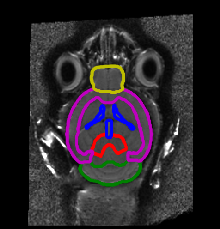
\includegraphics[height=.24\textwidth]{figures/atlas_overlays_dim-1pt6.png}
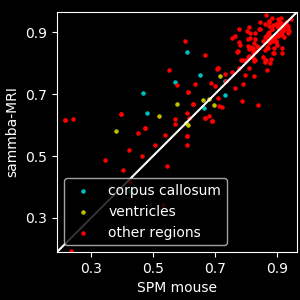
\includegraphics[height=.24\textwidth]{figures/bil2_transfo_dice_boxplots.png}
\end{center}
\caption{Dice's coefficient per region and animal (left); typical registered mouse image with average atlas contours superimposed as coloured lines (right).}\label{fig:dices}
\end{figure}

\begin{figure}[h!]
\begin{center}
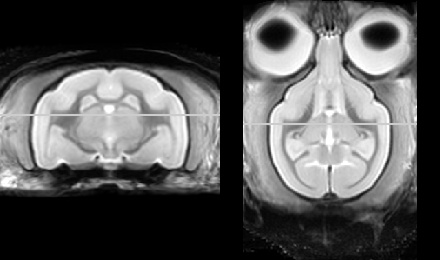
\includegraphics[width=.95\linewidth]{figures/sfn_template.jpg}
\end{center}
\caption{Mouse template.}\label{fig:mouse_template}
\end{figure}

\begin{figure}[h!]
\begin{center}
\includegraphics[height=.24\textwidth]{figures/mean_cbf_mricron2.png}
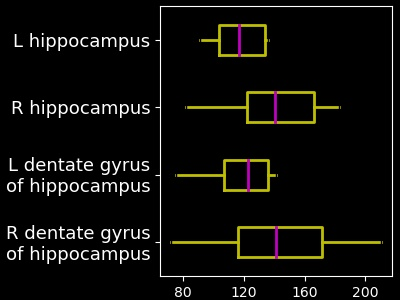
\includegraphics[height=.24\textwidth]{figures/regional_cbf_4rois_black_bg.jpg}
\end{center}
\caption{Group   average   CBF   map (left); individual regional CBF in ml/100g/min (right)}\label{fig:cbf}
\end{figure}

\begin{figure}[h!]
\begin{center}
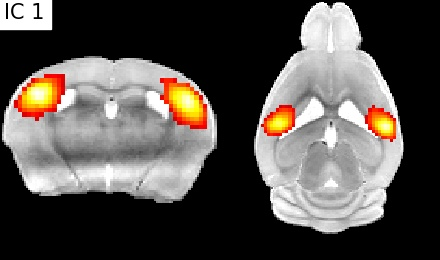
\includegraphics[width=0.45\linewidth]{{figures/component1.jpg}}
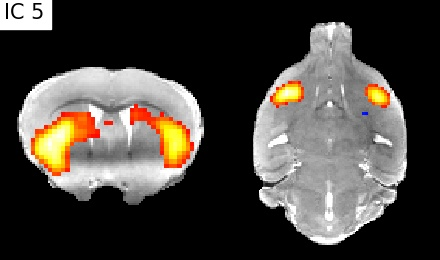
\includegraphics[width=0.45\linewidth]{{figures/component5.jpg}}
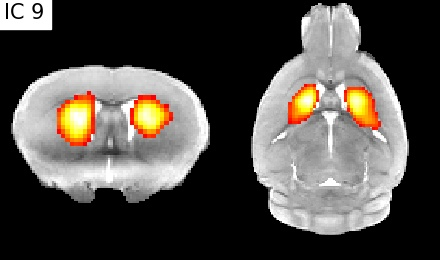
\includegraphics[width=0.45\linewidth]{{figures/component9.jpg}}
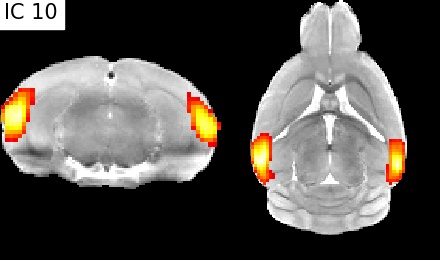
\includegraphics[width=0.45\linewidth]{{figures/component10.jpg}}
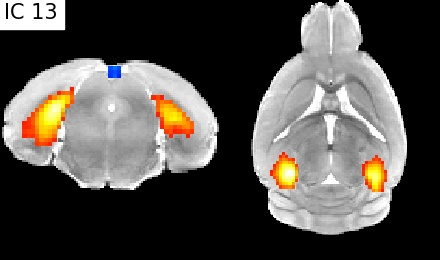
\includegraphics[width=0.45\linewidth]{{figures/component13.jpg}}
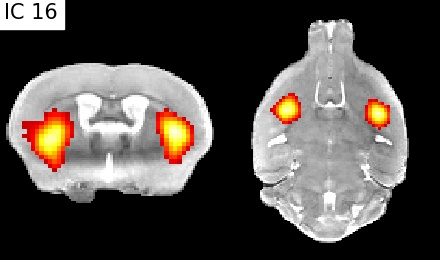
\includegraphics[width=0.45\linewidth]{{figures/component16.jpg}}
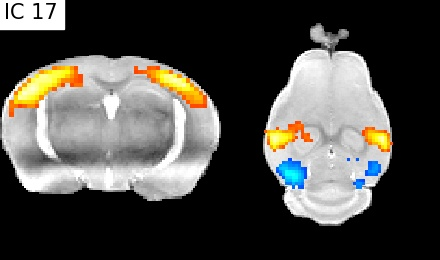
\includegraphics[width=0.45\linewidth]{{figures/component17.jpg}}
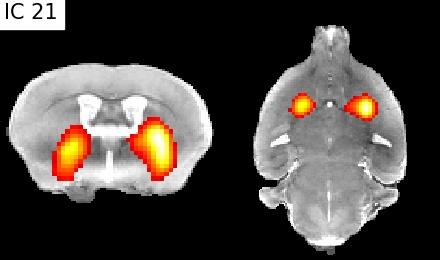
\includegraphics[width=0.45\linewidth]{{figures/component21.jpg}}
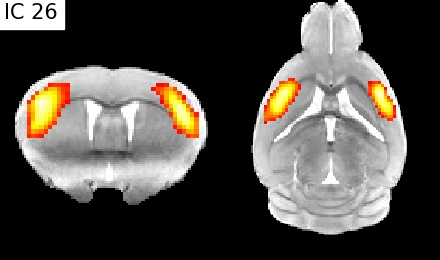
\includegraphics[width=0.45\linewidth]{{figures/component26.jpg}}
\end{center}
\caption{Bilateral ICA components}
\label{fig:ica}
\end{figure}


%\begin{figure}[h!]
%\begin{center}
%\includegraphics[width=15cm]{logos}
%\end{center}
%\caption{This is a figure with sub figures, \textbf{(A)} is one logo, \textbf{(B)} is a different logo.}\label{fig:2}
%\end{figure}

%%% If you are submitting a figure with subfigures please combine these into one image file with part labels integrated.
%%% If you don't add the figures in the LaTeX files, please upload them when submitting the article.
%%% Frontiers will add the figures at the end of the provisional pdf automatically
%%% The use of LaTeX coding to draw Diagrams/Figures/Structures should be avoided. They should be external callouts including graphics.

\end{document}
